
%(BEGIN_QUESTION)
% Copyright 2007, Tony R. Kuphaldt, released under the Creative Commons Attribution License (v 1.0)
% This means you may do almost anything with this work of mine, so long as you give me proper credit

Suppose this process is optimally tuned, with a measurement range of 0$^{o}$ F to 100$^{o}$ F:

$$\includegraphics[width=15.5cm]{i01643x01.eps}$$

Then, one day the decision is made to re-range the temperature transmitter (TT) for greater resolution: 50$^{o}$ F to 70$^{o}$ F instead of 0$^{o}$ F to 100$^{o}$ F.  As a result of this range-change, the process begins to oscillate around setpoint rather than hold steady at setpoint as it used to.

\vskip 10pt

Explain why this range-change caused the process control to become unstable, and propose a solution that will restore the previous quality of control.

\vfil 

\underbar{file i01643}
\eject
%(END_QUESTION)





%(BEGIN_ANSWER)

This is a graded question -- no answers or hints given!

%(END_ANSWER)





%(BEGIN_NOTES)

The range-change effectively increased the process gain five-fold.  With a transmitter range that is 5 times narrower (the new span is 20$^{o}$ F, from an old span of 100$^{o}$ F), the controller will see a process variable (PV) signal that is 5 times as sensitive to changes in process temperature than before.  In order to prevent the controller from over-reacting to changes in PV, the controller's aggressiveness must be correspondingly reduced by a factor of 5.

\vskip 10pt

When the gain of a control loop is changed as a result of changing transmitter span, valve C$_{v}$, or some other gain-altering aspect of the process, {\it all} control terms of the controller must be inversely altered (P, I, {\it and} D), not just the ``P'' term.  

A controller using either the {\it ideal} or the {\it series} equation would be easier to re-tune for changes in overall loop gain than a controller based on the {\it parallel} equation, because one tuning constant (K$_{c}$) proportionately impacts all three control terms.  With the {\it parallel} equation, all three tuning constants would have to be adjusted to achieve the same quality of control as before.  

There is no difference in ease of re-tuning between the {\it ideal} and {\it series} equations for a scenario such as this.

%INDEX% Control, proportional + integral + derivative: ideal (ISA) equation
%INDEX% Control, proportional + integral + derivative: parallel equation
%INDEX% Control, proportional + integral + derivative: series equation
%INDEX% Process: heat exchanger temperature control (generic)

%(END_NOTES)


